% Options for packages loaded elsewhere
\PassOptionsToPackage{unicode}{hyperref}
\PassOptionsToPackage{hyphens}{url}
%
\documentclass[
]{article}
\usepackage{amsmath,amssymb}
\usepackage{iftex}
\ifPDFTeX
  \usepackage[T1]{fontenc}
  \usepackage[utf8]{inputenc}
  \usepackage{textcomp} % provide euro and other symbols
\else % if luatex or xetex
  \usepackage{unicode-math} % this also loads fontspec
  \defaultfontfeatures{Scale=MatchLowercase}
  \defaultfontfeatures[\rmfamily]{Ligatures=TeX,Scale=1}
\fi
\usepackage{lmodern}
\ifPDFTeX\else
  % xetex/luatex font selection
\fi
% Use upquote if available, for straight quotes in verbatim environments
\IfFileExists{upquote.sty}{\usepackage{upquote}}{}
\IfFileExists{microtype.sty}{% use microtype if available
  \usepackage[]{microtype}
  \UseMicrotypeSet[protrusion]{basicmath} % disable protrusion for tt fonts
}{}
\makeatletter
\@ifundefined{KOMAClassName}{% if non-KOMA class
  \IfFileExists{parskip.sty}{%
    \usepackage{parskip}
  }{% else
    \setlength{\parindent}{0pt}
    \setlength{\parskip}{6pt plus 2pt minus 1pt}}
}{% if KOMA class
  \KOMAoptions{parskip=half}}
\makeatother
\usepackage{xcolor}
\usepackage[margin=1in]{geometry}
\usepackage{color}
\usepackage{fancyvrb}
\newcommand{\VerbBar}{|}
\newcommand{\VERB}{\Verb[commandchars=\\\{\}]}
\DefineVerbatimEnvironment{Highlighting}{Verbatim}{commandchars=\\\{\}}
% Add ',fontsize=\small' for more characters per line
\usepackage{framed}
\definecolor{shadecolor}{RGB}{248,248,248}
\newenvironment{Shaded}{\begin{snugshade}}{\end{snugshade}}
\newcommand{\AlertTok}[1]{\textcolor[rgb]{0.94,0.16,0.16}{#1}}
\newcommand{\AnnotationTok}[1]{\textcolor[rgb]{0.56,0.35,0.01}{\textbf{\textit{#1}}}}
\newcommand{\AttributeTok}[1]{\textcolor[rgb]{0.13,0.29,0.53}{#1}}
\newcommand{\BaseNTok}[1]{\textcolor[rgb]{0.00,0.00,0.81}{#1}}
\newcommand{\BuiltInTok}[1]{#1}
\newcommand{\CharTok}[1]{\textcolor[rgb]{0.31,0.60,0.02}{#1}}
\newcommand{\CommentTok}[1]{\textcolor[rgb]{0.56,0.35,0.01}{\textit{#1}}}
\newcommand{\CommentVarTok}[1]{\textcolor[rgb]{0.56,0.35,0.01}{\textbf{\textit{#1}}}}
\newcommand{\ConstantTok}[1]{\textcolor[rgb]{0.56,0.35,0.01}{#1}}
\newcommand{\ControlFlowTok}[1]{\textcolor[rgb]{0.13,0.29,0.53}{\textbf{#1}}}
\newcommand{\DataTypeTok}[1]{\textcolor[rgb]{0.13,0.29,0.53}{#1}}
\newcommand{\DecValTok}[1]{\textcolor[rgb]{0.00,0.00,0.81}{#1}}
\newcommand{\DocumentationTok}[1]{\textcolor[rgb]{0.56,0.35,0.01}{\textbf{\textit{#1}}}}
\newcommand{\ErrorTok}[1]{\textcolor[rgb]{0.64,0.00,0.00}{\textbf{#1}}}
\newcommand{\ExtensionTok}[1]{#1}
\newcommand{\FloatTok}[1]{\textcolor[rgb]{0.00,0.00,0.81}{#1}}
\newcommand{\FunctionTok}[1]{\textcolor[rgb]{0.13,0.29,0.53}{\textbf{#1}}}
\newcommand{\ImportTok}[1]{#1}
\newcommand{\InformationTok}[1]{\textcolor[rgb]{0.56,0.35,0.01}{\textbf{\textit{#1}}}}
\newcommand{\KeywordTok}[1]{\textcolor[rgb]{0.13,0.29,0.53}{\textbf{#1}}}
\newcommand{\NormalTok}[1]{#1}
\newcommand{\OperatorTok}[1]{\textcolor[rgb]{0.81,0.36,0.00}{\textbf{#1}}}
\newcommand{\OtherTok}[1]{\textcolor[rgb]{0.56,0.35,0.01}{#1}}
\newcommand{\PreprocessorTok}[1]{\textcolor[rgb]{0.56,0.35,0.01}{\textit{#1}}}
\newcommand{\RegionMarkerTok}[1]{#1}
\newcommand{\SpecialCharTok}[1]{\textcolor[rgb]{0.81,0.36,0.00}{\textbf{#1}}}
\newcommand{\SpecialStringTok}[1]{\textcolor[rgb]{0.31,0.60,0.02}{#1}}
\newcommand{\StringTok}[1]{\textcolor[rgb]{0.31,0.60,0.02}{#1}}
\newcommand{\VariableTok}[1]{\textcolor[rgb]{0.00,0.00,0.00}{#1}}
\newcommand{\VerbatimStringTok}[1]{\textcolor[rgb]{0.31,0.60,0.02}{#1}}
\newcommand{\WarningTok}[1]{\textcolor[rgb]{0.56,0.35,0.01}{\textbf{\textit{#1}}}}
\usepackage{graphicx}
\makeatletter
\def\maxwidth{\ifdim\Gin@nat@width>\linewidth\linewidth\else\Gin@nat@width\fi}
\def\maxheight{\ifdim\Gin@nat@height>\textheight\textheight\else\Gin@nat@height\fi}
\makeatother
% Scale images if necessary, so that they will not overflow the page
% margins by default, and it is still possible to overwrite the defaults
% using explicit options in \includegraphics[width, height, ...]{}
\setkeys{Gin}{width=\maxwidth,height=\maxheight,keepaspectratio}
% Set default figure placement to htbp
\makeatletter
\def\fps@figure{htbp}
\makeatother
\setlength{\emergencystretch}{3em} % prevent overfull lines
\providecommand{\tightlist}{%
  \setlength{\itemsep}{0pt}\setlength{\parskip}{0pt}}
\setcounter{secnumdepth}{-\maxdimen} % remove section numbering
\ifLuaTeX
  \usepackage{selnolig}  % disable illegal ligatures
\fi
\IfFileExists{bookmark.sty}{\usepackage{bookmark}}{\usepackage{hyperref}}
\IfFileExists{xurl.sty}{\usepackage{xurl}}{} % add URL line breaks if available
\urlstyle{same}
\hypersetup{
  pdftitle={Ejercicio 7},
  hidelinks,
  pdfcreator={LaTeX via pandoc}}

\title{Ejercicio 7}
\author{}
\date{\vspace{-2.5em}}

\begin{document}
\maketitle

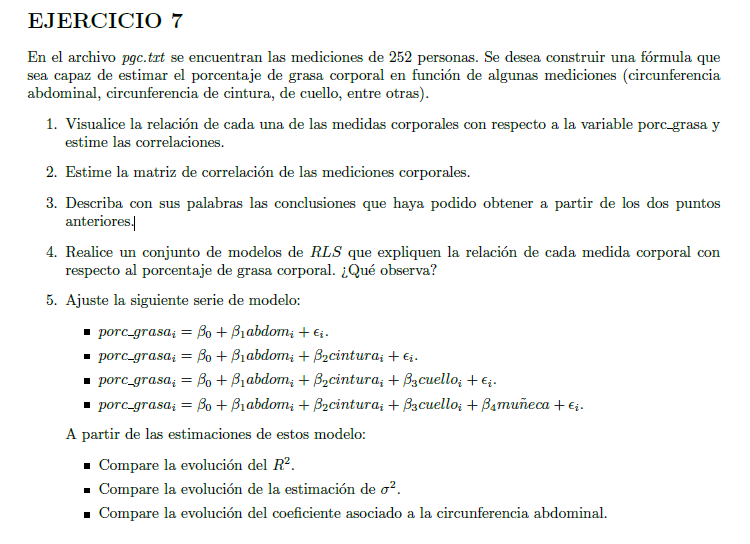
\includegraphics{pauta 7.png}

\begin{verbatim}
## corrplot 0.92 loaded
\end{verbatim}

\begin{enumerate}
\def\labelenumi{\arabic{enumi}.}
\tightlist
\item
  Visualice la relacion de cada una de las medidas corporales con
  respecto a la variable porc\_grasa y estime las correlaciones
\end{enumerate}

\begin{Shaded}
\begin{Highlighting}[]
\NormalTok{mod }\OtherTok{\textless{}{-}} \FunctionTok{lm}\NormalTok{(porc\_grasa }\SpecialCharTok{\textasciitilde{}}\NormalTok{ cuello }\SpecialCharTok{+}\NormalTok{ pecho }\SpecialCharTok{+}\NormalTok{ abdomen }\SpecialCharTok{+}\NormalTok{ cadera }\SpecialCharTok{+}\NormalTok{ muslo}
          \SpecialCharTok{+}\NormalTok{ rodilla }\SpecialCharTok{+}\NormalTok{ tobillo }\SpecialCharTok{+}\NormalTok{ biceps }\SpecialCharTok{+}\NormalTok{ brazo }\SpecialCharTok{+}\NormalTok{ muneca, }\AttributeTok{data =}\NormalTok{ datos )}

\FunctionTok{summary}\NormalTok{(mod) }
\end{Highlighting}
\end{Shaded}

\begin{verbatim}
## 
## Call:
## lm(formula = porc_grasa ~ cuello + pecho + abdomen + cadera + 
##     muslo + rodilla + tobillo + biceps + brazo + muneca, data = datos)
## 
## Residuals:
##     Min      1Q  Median      3Q     Max 
## -9.3159 -2.7435 -0.1584  2.8388 10.5150 
## 
## Coefficients:
##              Estimate Std. Error t value Pr(>|t|)    
## (Intercept)  7.228749   6.214309   1.163  0.24588    
## cuello      -0.581947   0.208580  -2.790  0.00569 ** 
## pecho       -0.090847   0.085430  -1.063  0.28866    
## abdomen      0.960229   0.071582  13.414  < 2e-16 ***
## cadera      -0.391355   0.112686  -3.473  0.00061 ***
## muslo        0.133708   0.124922   1.070  0.28554    
## rodilla     -0.094055   0.212394  -0.443  0.65828    
## tobillo      0.004222   0.203175   0.021  0.98344    
## biceps       0.111196   0.159118   0.699  0.48533    
## brazo        0.344536   0.185511   1.857  0.06450 .  
## muneca      -1.353472   0.471410  -2.871  0.00445 ** 
## ---
## Signif. codes:  0 '***' 0.001 '**' 0.01 '*' 0.05 '.' 0.1 ' ' 1
## 
## Residual standard error: 4.071 on 241 degrees of freedom
## Multiple R-squared:  0.7351, Adjusted R-squared:  0.7241 
## F-statistic: 66.87 on 10 and 241 DF,  p-value: < 2.2e-16
\end{verbatim}

\begin{enumerate}
\def\labelenumi{\arabic{enumi}.}
\setcounter{enumi}{1}
\tightlist
\item
  Estime la matriz de correlacion de las mediciones corporales.
\end{enumerate}

\begin{Shaded}
\begin{Highlighting}[]
\CommentTok{\#Matriz de correlaciones}



\NormalTok{analisis }\OtherTok{\textless{}{-}}\NormalTok{ datos[,}\SpecialCharTok{{-}}\NormalTok{(}\FunctionTok{c}\NormalTok{(}\DecValTok{2}\NormalTok{,}\DecValTok{3}\NormalTok{,}\DecValTok{4}\NormalTok{))]}


\NormalTok{correlacion }\OtherTok{\textless{}{-}} \FunctionTok{round}\NormalTok{(}\FunctionTok{cor}\NormalTok{(analisis),}\DecValTok{3}\NormalTok{)}

\FunctionTok{corrplot}\NormalTok{(correlacion, }\AttributeTok{method=}\StringTok{"circle"}\NormalTok{, }\AttributeTok{type=}\StringTok{"upper"}\NormalTok{,}\AttributeTok{pch.col =} \DecValTok{10}\NormalTok{)}
\end{Highlighting}
\end{Shaded}

\includegraphics{Ejercicio-7_files/figure-latex/unnamed-chunk-3-1.pdf}
3. Describa con sus palabras las conclusiones que haya podido obtener a
partir de los dos puntos anteriores.

Las variables están corelacionadas de manera positiva, lo cual tiene
sentido al menos desde una noción más biológica donde si una parte del
cuerpo es de un tamaño la otra guardará cierta proporción, así mismo se
observa que es el tamaño del tobillo la que menos incide en las otras
variables.

Por otra parte, el modelo del punto uno, explica en un 73,5\% el
porcentaje de grasa corporal, siendo cadera, cuello, abdomen, y muñeca
las que más información arrojan sobre el modelo en sí.

\begin{enumerate}
\def\labelenumi{\arabic{enumi}.}
\setcounter{enumi}{3}
\tightlist
\item
  Realice un conjunto de modelos de RLS que expliquen la relacion de
  cada medida corporal con respecto al porcentaje de grasa corporal.
  ¿Que observa?
\end{enumerate}

\begin{Shaded}
\begin{Highlighting}[]
\NormalTok{mod1 }\OtherTok{\textless{}{-}} \FunctionTok{lm}\NormalTok{(porc\_grasa }\SpecialCharTok{\textasciitilde{}}\NormalTok{ cuello , }\AttributeTok{data =}\NormalTok{ datos )}

\NormalTok{mod2 }\OtherTok{\textless{}{-}} \FunctionTok{lm}\NormalTok{(porc\_grasa }\SpecialCharTok{\textasciitilde{}}\NormalTok{  pecho , }\AttributeTok{data =}\NormalTok{ datos )}

\NormalTok{mod3 }\OtherTok{\textless{}{-}} \FunctionTok{lm}\NormalTok{(porc\_grasa }\SpecialCharTok{\textasciitilde{}}\NormalTok{  abdomen , }\AttributeTok{data =}\NormalTok{ datos )}

\NormalTok{mod4 }\OtherTok{\textless{}{-}} \FunctionTok{lm}\NormalTok{(porc\_grasa }\SpecialCharTok{\textasciitilde{}}\NormalTok{  cadera , }\AttributeTok{data =}\NormalTok{ datos )}

\NormalTok{mod5}\OtherTok{\textless{}{-}} \FunctionTok{lm}\NormalTok{(porc\_grasa }\SpecialCharTok{\textasciitilde{}}\NormalTok{  muslo , }\AttributeTok{data =}\NormalTok{ datos )}

\NormalTok{mod6}\OtherTok{\textless{}{-}} \FunctionTok{lm}\NormalTok{(porc\_grasa }\SpecialCharTok{\textasciitilde{}}\NormalTok{  rodilla , }\AttributeTok{data =}\NormalTok{ datos )}

\NormalTok{mod7}\OtherTok{\textless{}{-}} \FunctionTok{lm}\NormalTok{(porc\_grasa }\SpecialCharTok{\textasciitilde{}}\NormalTok{  tobillo , }\AttributeTok{data =}\NormalTok{ datos )}

\NormalTok{mod8}\OtherTok{\textless{}{-}} \FunctionTok{lm}\NormalTok{(porc\_grasa }\SpecialCharTok{\textasciitilde{}}\NormalTok{  biceps , }\AttributeTok{data =}\NormalTok{ datos )}

\NormalTok{mod9}\OtherTok{\textless{}{-}} \FunctionTok{lm}\NormalTok{(porc\_grasa }\SpecialCharTok{\textasciitilde{}}\NormalTok{  brazo , }\AttributeTok{data =}\NormalTok{ datos )}

\NormalTok{mod10}\OtherTok{\textless{}{-}} \FunctionTok{lm}\NormalTok{(porc\_grasa }\SpecialCharTok{\textasciitilde{}}\NormalTok{  muneca , }\AttributeTok{data =}\NormalTok{ datos )}

\NormalTok{algo }\OtherTok{\textless{}{-}} \FunctionTok{rbind}\NormalTok{(}\FunctionTok{coef}\NormalTok{(mod1),}\FunctionTok{coef}\NormalTok{(mod2),}\FunctionTok{coef}\NormalTok{(mod3),}\FunctionTok{coef}\NormalTok{(mod4),}\FunctionTok{coef}\NormalTok{(mod5),}\FunctionTok{coef}\NormalTok{(mod6)}
\NormalTok{      ,}\FunctionTok{coef}\NormalTok{(mod7),}\FunctionTok{coef}\NormalTok{(mod8),}\FunctionTok{coef}\NormalTok{(mod9),}\FunctionTok{coef}\NormalTok{(mod10))}

\NormalTok{algo }\OtherTok{\textless{}{-}}\NormalTok{ algo[,}\DecValTok{2}\NormalTok{]}

\NormalTok{RLS\_porcGrasa }\OtherTok{\textless{}{-}} \FunctionTok{as.data.frame}\NormalTok{(}\FunctionTok{cbind}\NormalTok{(}\FunctionTok{c}\NormalTok{(}\StringTok{"Cuello"}\NormalTok{,}\StringTok{"Pecho"}\NormalTok{,}\StringTok{"Abdomen"}\NormalTok{,}\StringTok{"Cadera"}\NormalTok{,}\StringTok{"Muslo"}\NormalTok{,}\StringTok{"Rodilla"}\NormalTok{,}\StringTok{"Tobillo"}\NormalTok{,}\StringTok{"Biceps"}\NormalTok{,}\StringTok{"Brazo"}\NormalTok{,}\StringTok{"Muñeca"}\NormalTok{),algo))}

\FunctionTok{colnames}\NormalTok{(RLS\_porcGrasa)}\OtherTok{\textless{}{-}}\FunctionTok{c}\NormalTok{(}\StringTok{"Variable"}\NormalTok{,}\StringTok{"Beta"}\NormalTok{)}

\FunctionTok{class}\NormalTok{(RLS\_porcGrasa)}
\end{Highlighting}
\end{Shaded}

\begin{verbatim}
## [1] "data.frame"
\end{verbatim}

\begin{Shaded}
\begin{Highlighting}[]
\NormalTok{RLS\_porcGrasa }\OtherTok{\textless{}{-}}\NormalTok{ RLS\_porcGrasa[}\FunctionTok{order}\NormalTok{(RLS\_porcGrasa}\SpecialCharTok{$}\NormalTok{Beta,}\AttributeTok{decreasing =}\NormalTok{ T),]}

\NormalTok{RLS\_porcGrasa}
\end{Highlighting}
\end{Shaded}

\begin{verbatim}
##    Variable              Beta
## 10   Muñeca  2.88563598657192
## 6   Rodilla  1.63187973004883
## 1    Cuello   1.5670899630347
## 9     Brazo  1.39343956604193
## 8    Biceps  1.26483448827388
## 7   Tobillo  1.22001365754821
## 5     Muslo 0.828661701987687
## 4    Cadera 0.676950137461153
## 2     Pecho 0.646222311718054
## 3   Abdomen 0.584890527012418
\end{verbatim}

\begin{Shaded}
\begin{Highlighting}[]
\CommentTok{\#abdomen\_grafico \textless{}{-} ggplot(data = datos, mapping = aes(x=porc\_grasa,y=abdomen))+geom\_point()+ylab("Centimetros de abdomen")+xlab("Porcentaje de grasa")+labs(title = "Relación centrímetros de abdomen{-}Porcentaje grasa corporal",caption = "R{-}squared:  0.6621")}


\CommentTok{\#muneca\_grafico \textless{}{-} ggplot(data = datos, mapping = aes(x=porc\_grasa,y=muneca))+geom\_point()+ylab("Centimetros de muneca")+xlab("Porcentaje de grasa")+labs(title = "Relación centrímetros de muñeca{-}Porcentaje grasa corporal", caption = "R{-}squared:  0.1208")}


\NormalTok{RLS\_porcGrasa}
\end{Highlighting}
\end{Shaded}

\begin{verbatim}
##    Variable              Beta
## 10   Muñeca  2.88563598657192
## 6   Rodilla  1.63187973004883
## 1    Cuello   1.5670899630347
## 9     Brazo  1.39343956604193
## 8    Biceps  1.26483448827388
## 7   Tobillo  1.22001365754821
## 5     Muslo 0.828661701987687
## 4    Cadera 0.676950137461153
## 2     Pecho 0.646222311718054
## 3   Abdomen 0.584890527012418
\end{verbatim}

\begin{Shaded}
\begin{Highlighting}[]
\FunctionTok{summary}\NormalTok{(mod3)}
\end{Highlighting}
\end{Shaded}

\begin{verbatim}
## 
## Call:
## lm(formula = porc_grasa ~ abdomen, data = datos)
## 
## Residuals:
##      Min       1Q   Median       3Q      Max 
## -17.6257  -3.4672   0.0111   3.1415  11.9754 
## 
## Coefficients:
##              Estimate Std. Error t value Pr(>|t|)    
## (Intercept) -35.19661    2.46229  -14.29   <2e-16 ***
## abdomen       0.58489    0.02643   22.13   <2e-16 ***
## ---
## Signif. codes:  0 '***' 0.001 '**' 0.01 '*' 0.05 '.' 0.1 ' ' 1
## 
## Residual standard error: 4.514 on 250 degrees of freedom
## Multiple R-squared:  0.6621, Adjusted R-squared:  0.6608 
## F-statistic: 489.9 on 1 and 250 DF,  p-value: < 2.2e-16
\end{verbatim}

\begin{Shaded}
\begin{Highlighting}[]
\CommentTok{\#abdomen\_grafico}

\FunctionTok{summary}\NormalTok{(mod10)}
\end{Highlighting}
\end{Shaded}

\begin{verbatim}
## 
## Call:
## lm(formula = porc_grasa ~ muneca, data = datos)
## 
## Residuals:
##      Min       1Q   Median       3Q      Max 
## -14.8183  -5.5840   0.1231   5.0703  25.6703 
## 
## Coefficients:
##             Estimate Std. Error t value Pr(>|t|)    
## (Intercept) -33.6660     8.9870  -3.746 0.000223 ***
## muneca        2.8856     0.4923   5.861 1.45e-08 ***
## ---
## Signif. codes:  0 '***' 0.001 '**' 0.01 '*' 0.05 '.' 0.1 ' ' 1
## 
## Residual standard error: 7.282 on 250 degrees of freedom
## Multiple R-squared:  0.1208, Adjusted R-squared:  0.1173 
## F-statistic: 34.35 on 1 and 250 DF,  p-value: 1.446e-08
\end{verbatim}

\begin{Shaded}
\begin{Highlighting}[]
\CommentTok{\#muneca\_grafico}
\end{Highlighting}
\end{Shaded}

Según este resumen de datos, cada variable tiene una relación positiva
con el porcentaje de grasa. Pondremos particular atención en las
variables abdomen y muñeca.

Para el caso de abdomen, el incremento de un punto porcentual de grasa
corporal implica el aumento de medio centímetro de abdomen, mientras que
para la medida de muñeca representa un incremento de 2.8 centímetros.
Por otra parte, explicar el porcentaje de grasa corporal mediante la
medida de abdomen es más confiable que por el de la muñeca, ya que entre
otras cosas, el coeficiente R2 es de 66.2\% para el primero y de 12.1\%
para el segundo

\begin{enumerate}
\def\labelenumi{\arabic{enumi}.}
\setcounter{enumi}{4}
\tightlist
\item
  Ajuste la siguiente serie de modelo:
\end{enumerate}

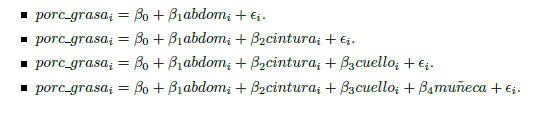
\includegraphics{pauta 5.png}

A partir de las estimaciones de estos modelo:

Compare la evolucion del R2.

Compare la evolucion de la estimacion de sigma2.

Compare la evolucion del coefiente asociado a la circunferencia
abdominal.

\begin{Shaded}
\begin{Highlighting}[]
\NormalTok{mod11}\OtherTok{\textless{}{-}} \FunctionTok{lm}\NormalTok{(porc\_grasa }\SpecialCharTok{\textasciitilde{}}\NormalTok{  abdomen , }\AttributeTok{data =}\NormalTok{ datos )}

\FunctionTok{summary}\NormalTok{(mod11)}
\end{Highlighting}
\end{Shaded}

\begin{verbatim}
## 
## Call:
## lm(formula = porc_grasa ~ abdomen, data = datos)
## 
## Residuals:
##      Min       1Q   Median       3Q      Max 
## -17.6257  -3.4672   0.0111   3.1415  11.9754 
## 
## Coefficients:
##              Estimate Std. Error t value Pr(>|t|)    
## (Intercept) -35.19661    2.46229  -14.29   <2e-16 ***
## abdomen       0.58489    0.02643   22.13   <2e-16 ***
## ---
## Signif. codes:  0 '***' 0.001 '**' 0.01 '*' 0.05 '.' 0.1 ' ' 1
## 
## Residual standard error: 4.514 on 250 degrees of freedom
## Multiple R-squared:  0.6621, Adjusted R-squared:  0.6608 
## F-statistic: 489.9 on 1 and 250 DF,  p-value: < 2.2e-16
\end{verbatim}

\begin{Shaded}
\begin{Highlighting}[]
\NormalTok{mod12}\OtherTok{\textless{}{-}} \FunctionTok{lm}\NormalTok{(porc\_grasa }\SpecialCharTok{\textasciitilde{}}\NormalTok{  abdomen }\SpecialCharTok{+}\NormalTok{ cadera , }\AttributeTok{data =}\NormalTok{ datos )}

\FunctionTok{summary}\NormalTok{(mod12)}
\end{Highlighting}
\end{Shaded}

\begin{verbatim}
## 
## Call:
## lm(formula = porc_grasa ~ abdomen + cadera, data = datos)
## 
## Residuals:
##     Min      1Q  Median      3Q     Max 
## -11.532  -3.153  -0.256   2.953  11.746 
## 
## Coefficients:
##              Estimate Std. Error t value Pr(>|t|)    
## (Intercept) -17.09863    4.30711  -3.970 9.41e-05 ***
## abdomen       0.81259    0.05194  15.644  < 2e-16 ***
## cadera       -0.39210    0.07818  -5.015 1.01e-06 ***
## ---
## Signif. codes:  0 '***' 0.001 '**' 0.01 '*' 0.05 '.' 0.1 ' ' 1
## 
## Residual standard error: 4.311 on 249 degrees of freedom
## Multiple R-squared:  0.6931, Adjusted R-squared:  0.6907 
## F-statistic: 281.2 on 2 and 249 DF,  p-value: < 2.2e-16
\end{verbatim}

\begin{Shaded}
\begin{Highlighting}[]
\NormalTok{mod13}\OtherTok{\textless{}{-}} \FunctionTok{lm}\NormalTok{(porc\_grasa }\SpecialCharTok{\textasciitilde{}}\NormalTok{  abdomen }\SpecialCharTok{+}\NormalTok{ cadera }\SpecialCharTok{+}\NormalTok{ cuello , }\AttributeTok{data =}\NormalTok{ datos )}

\FunctionTok{summary}\NormalTok{(mod13)}
\end{Highlighting}
\end{Shaded}

\begin{verbatim}
## 
## Call:
## lm(formula = porc_grasa ~ abdomen + cadera + cuello, data = datos)
## 
## Residuals:
##     Min      1Q  Median      3Q     Max 
## -9.9972 -2.9498 -0.1737  2.8267 12.4451 
## 
## Coefficients:
##             Estimate Std. Error t value Pr(>|t|)    
## (Intercept) -4.33037    5.07977  -0.852    0.395    
## abdomen      0.89166    0.05330  16.728  < 2e-16 ***
## cadera      -0.31127    0.07771  -4.006 8.18e-05 ***
## cuello      -0.74128    0.16939  -4.376 1.78e-05 ***
## ---
## Signif. codes:  0 '***' 0.001 '**' 0.01 '*' 0.05 '.' 0.1 ' ' 1
## 
## Residual standard error: 4.162 on 248 degrees of freedom
## Multiple R-squared:  0.7151, Adjusted R-squared:  0.7117 
## F-statistic: 207.5 on 3 and 248 DF,  p-value: < 2.2e-16
\end{verbatim}

\begin{Shaded}
\begin{Highlighting}[]
\NormalTok{mod14}\OtherTok{\textless{}{-}} \FunctionTok{lm}\NormalTok{(porc\_grasa }\SpecialCharTok{\textasciitilde{}}\NormalTok{  abdomen }\SpecialCharTok{+}\NormalTok{ cadera }\SpecialCharTok{+}\NormalTok{ cuello }\SpecialCharTok{+}\NormalTok{ muneca , }\AttributeTok{data =}\NormalTok{ datos )}

\FunctionTok{summary}\NormalTok{(mod14)}
\end{Highlighting}
\end{Shaded}

\begin{verbatim}
## 
## Call:
## lm(formula = porc_grasa ~ abdomen + cadera + cuello + muneca, 
##     data = datos)
## 
## Residuals:
##      Min       1Q   Median       3Q      Max 
## -11.3584  -2.7101  -0.2303   2.9092  10.9033 
## 
## Coefficients:
##             Estimate Std. Error t value Pr(>|t|)    
## (Intercept)  4.65504    5.79616   0.803 0.422675    
## abdomen      0.89202    0.05243  17.014  < 2e-16 ***
## cadera      -0.28141    0.07705  -3.652 0.000317 ***
## cuello      -0.43807    0.19388  -2.260 0.024722 *  
## muneca      -1.29023    0.42188  -3.058 0.002471 ** 
## ---
## Signif. codes:  0 '***' 0.001 '**' 0.01 '*' 0.05 '.' 0.1 ' ' 1
## 
## Residual standard error: 4.094 on 247 degrees of freedom
## Multiple R-squared:  0.7255, Adjusted R-squared:  0.7211 
## F-statistic: 163.2 on 4 and 247 DF,  p-value: < 2.2e-16
\end{verbatim}

\begin{Shaded}
\begin{Highlighting}[]
\NormalTok{comparación }\OtherTok{\textless{}{-}} \FunctionTok{as.data.frame}\NormalTok{(}\FunctionTok{cbind}\NormalTok{(}\FunctionTok{c}\NormalTok{(}\FloatTok{0.6621}\NormalTok{,}\FloatTok{0.6931}\NormalTok{,}\FloatTok{0.7151}\NormalTok{,}\FloatTok{0.7255}\NormalTok{),}
                                   \FunctionTok{c}\NormalTok{(}\FloatTok{4.514}\NormalTok{,}\FloatTok{4.311}\NormalTok{,}\FloatTok{4.162}\NormalTok{,}\FloatTok{4.094}\NormalTok{),}
                                   \FunctionTok{c}\NormalTok{(}\FloatTok{0.58489}\NormalTok{,}\FloatTok{0.81259}\NormalTok{,}\FloatTok{0.89166}\NormalTok{,}\FloatTok{0.89202}\NormalTok{)))}

\FunctionTok{colnames}\NormalTok{(comparación)}\OtherTok{\textless{}{-}}\FunctionTok{c}\NormalTok{(}\StringTok{"R{-}squared"}\NormalTok{,}\StringTok{"Residual standard error"}\NormalTok{,}\StringTok{"Beta\_abdomen"}\NormalTok{)}

\FunctionTok{rownames}\NormalTok{(comparación)}\OtherTok{\textless{}{-}}\FunctionTok{c}\NormalTok{(}\StringTok{"Abdomen"}\NormalTok{,}\StringTok{"Abdomen/Cadera"}\NormalTok{,}\StringTok{"Abdomen/Cadera/Cuello"}\NormalTok{,}\StringTok{"Abdomen/Cadera/Cuello/Muñeca"}\NormalTok{)}

\NormalTok{comparación}
\end{Highlighting}
\end{Shaded}

\begin{verbatim}
##                              R-squared Residual standard error Beta_abdomen
## Abdomen                         0.6621                   4.514      0.58489
## Abdomen/Cadera                  0.6931                   4.311      0.81259
## Abdomen/Cadera/Cuello           0.7151                   4.162      0.89166
## Abdomen/Cadera/Cuello/Muñeca    0.7255                   4.094      0.89202
\end{verbatim}

\end{document}
